\section*{جواب سوال ۵}

برای یک زنجیره مارکوف با استیت‌های \{1, 2, 3\} و ماتریس انتقال زیر:

\[
P = \begin{pmatrix}
	\frac{1}{4} & \frac{1}{4} & \frac{1}{2} \\
	\frac{1}{3} & 0 & \frac{2}{3} \\
	0 & \frac{1}{2} & \frac{1}{2}
\end{pmatrix}
\]

نمودار زنجیره مارکوف مربوط به این ماتریس به صورت زیر است:

\begin{figure}[H]
	\centering
	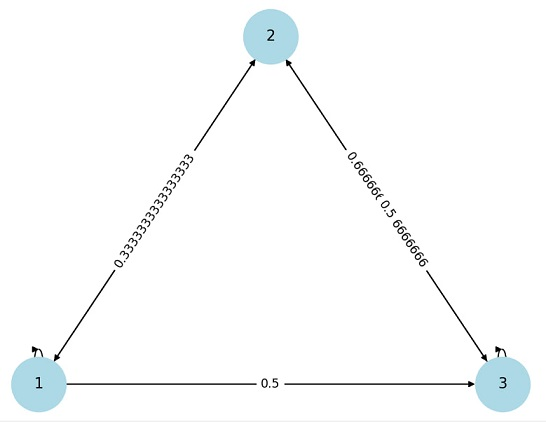
\includegraphics{pic1.jpg}
	\label{fig:label4}
\end{figure}

محاسبه احتمال \(P(X_1 = 3, X_2 = 2, X_3 = 1)\) بر اساس قانون زنجیره‌ای احتمال انجام می‌شود:

\[
P(X_1 = 3, X_2 = 2, X_3 = 1) = P(X_1 = 3) \times P_{32} \times P_{21}
\]

از آنجا که \(P(X_1 = 1) = P(X_1 = 2) = P(X_1 = 3) = \frac{1}{3}\)، محاسبه صحیح به صورت زیر خواهد بود:

\[
P(X_1 = 3, X_2 = 2, X_3 = 1) = \frac{1}{3} \times \frac{1}{2} \times \frac{1}{3} = \frac{1}{18}
\]